\section{Obtención de nombres de profesores} \label{nomProfesores}

En la simulación de solicitudes se eligen materias y horarios con respecto a los profesores. Es por ello que guardamos información de cada profesor. Definimos la matriz \textit{mat\_nom\_prof}, con 2 columnas.

En la primer columna se tienen los nombres de todos los profesores que han impartido clase desde el semestre 2015-1 hasta el 2020-1. Dichos nombres los obtuvimos de la matriz \textit{m\_grande\_2015}. Ésta es una submatriz de \textit{m\_grande\_total} con los datos de los semestres del 2015-1 al 2020-1.

En la segunda columna de \textit{mat\_nom\_prof} se tiene un $1$ si el profesor es de tiempo completo y un $0$ si es de asignatura. En las siguientes subsecciones veremos cómo llenamos esta columna y cómo hicimos la limpieza de los nombres de los profesores.

\subsection{Profesores de tiempo completo}

Para llenar la segunda columna de la matriz \textit{mat\_nom\_prof} ingresamos a la página \url{www.matematicas.unam.mx/index.php/nosotros/profesores-de-tiempo-completo}, del Departamento de Matemáticas. Con la aplicación \textit{SelectorGadget} seleccionamos uno de los nombres de los profesores de tiempo completo. En la \figurename{~\ref{profTC_SelectorGadget}} podemos ver el código CSS que utilizamos para obtener los datos en \textit{R}. También observamos que se seleccionaron 94 profesores.

\begin{figure}[H]
\centering
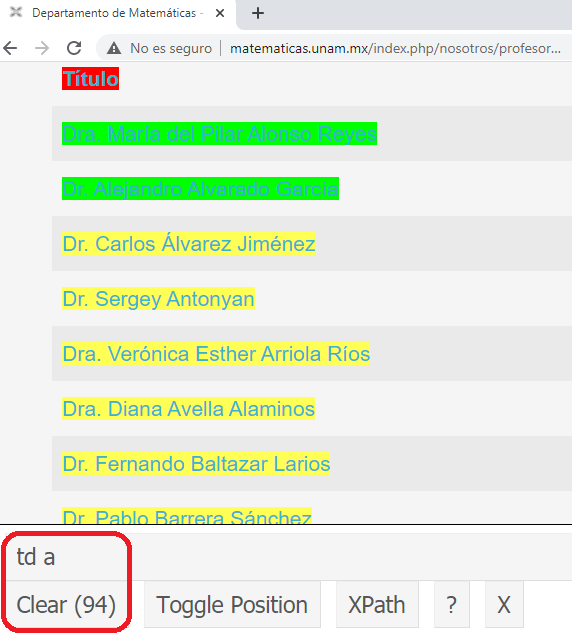
\includegraphics[scale = 0.8]{profesores_TC_SelectorGadget} %width=\textwidth
\caption[\textit{Profesores de tiempo completo: SelectorGadget}]{\textit{Se muestra la selección de profesores de tiempo completo con la aplicación SelectorGadget. Se puede ver el código CSS utilizado en R.}}\label{profTC_SelectorGadget}
\end{figure}

Al extraer la información en \textit{R} obtuvimos un vector con 94 entradas. En la \figurename{~\ref{profTC_sinLimpiar}} podemos ver los primeros 20 valores del vector. Notamos que cada entrada del vector inicia con los caracteres $\backslash n \backslash t \backslash t \backslash t \backslash t \backslash t \backslash t \backslash t$. Estos caracteres, en la presentación final de la página de internet, indican un salto de línea y las tabulaciones o espacios que se tienen de izquierda a derecha.

\begin{figure}[H]
\centering
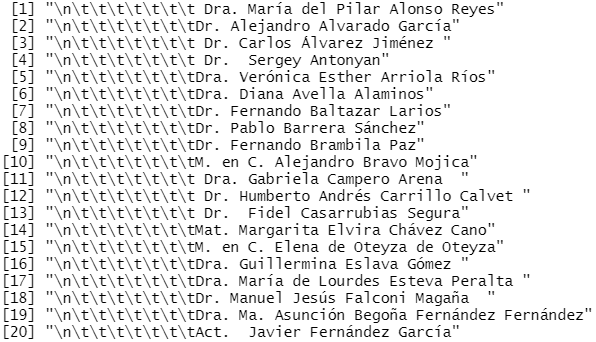
\includegraphics[scale = 0.8]{profesores_TC_sinLimpiar} %width=\textwidth
\caption[\textit{Vector de profesores de tiempo completo}]{\textit{Se observan las primeras 20 entradas del vector obtenido con la aplicación SelectorGadget. El vector contiene los nombres de los profesores de tiempo completo.}}\label{profTC_sinLimpiar}
\end{figure}

Limpiamos los datos para obtener un vector que sólo tuviera los nombres de los profesores, sin su título. Eliminamos el título porque en los horarios publicados en las páginas de la Facultad sus nombres no lo tienen. También eliminamos los espacios finales que había en algunos nombres.

De esta manera obtuvimos el vector con el nombre de los profesores de tiempo completo del Departamento de Matemáticas. Dicho vector lo comparamos con la primer columna de la matriz \textit{mat\_nom\_prof}. Cuando los nombres coincidieron, pusimos un $1$ en el renglón correspondiente.

Al limpiar los datos encontramos 11 nombres que analizamos de manera particular porque no aparecía el $1$ en su respectivo renglón. Encontramos que no aparecía la información necesaria en la matriz \textit{mat\_nom\_prof} por diferencias en los nombres. Encontramos diferencias por acentos, por mayúsculas y por nombres incompletos. En la \tablename{~\ref{DifNomProfTC}} vemos los nombres que aparecen en las páginas de la Facultad comparados con los que aparecen en la página del Departamento de Matemáticas.

\begin{table}[H]
\centering
\resizebox{\textwidth}{!}{%
  \begin{tabular}{|c|c|}
  \hline 
  \textbf{Nombre en páginas de la Facultad} & \textbf{Nombre en página del Depto. de Matemáticas} \\ 
  \hline 
  Alejandro Ricardo Garciadiego Dantan & Alejandro Ricardo Garciadiego Dantán \\ 
  \hline 
  Edith Corina Sáenz Valadez & Edith Corina Sáenz Valadéz \\ 
  \hline 
  Emilio Esteban Lluis Puebla & Emilio Lluis Puebla \\
  \hline 
  Guillermo Javier Francisco Sienra Loera & Guillermo Sienra Loera \\
  \hline 
  María Asunción Begoña Fernández Fernández & Ma. Asunción Begoña Fernández Fernández \\ 
  \hline 
  María Concepción Ana Luisa Solís González-Cosío & Ana Luisa Solís González Cosío \\ 
  \hline
  María Isabel Puga Espinosa & Isabel Puga Espinosa \\ 
  \hline 
  María Lourdes Velasco Arreguí & María de Lourdes Velasco Arregui \\ 
  \hline 
  Mucuy-Kak del Carmen Guevara Aguirre & Mucuy-kak del Carmen Guevara Aguirre \\ 
  \hline 
  Oscar Alfredo Palmas Velasco & Óscar Alfredo Palmas Velasco \\ 
  \hline 
  Úrsula Xiomara Iturrarán Viveros & Úrsula Iturrarán Viveros \\ 
  \hline 
  \end{tabular}
} 
\caption[\textit{Diferencias en nombres de profesores de tiempo completo}]{\textit{Se muestran los 11 nombres de los profesores de tiempo completo que se analizaron de manera individual. Se encontraron diferencias en acentos, mayúsculas y nombres incompletos.}}\label{DifNomProfTC}
\end{table}

\subsection{Profesores de asignatura}

Al llenar la matriz \textit{mat\_nom\_prof} con los nombres de los profesores vimos que la dimensión de dicha matriz es $1387 \times 2$. Por lo que tenemos 1387 nombres de profesores de los cuales 94 son profesores de tiempo completo. En esta subsección explicaremos cómo hicimos la limpieza de los nombres de los profesores de asignatura. Es decir los 1293 nombres que nos falta por analizar.

Lo primero que hicimos fue ordenar los nombres de los profesores de asignatura alfabéticamente. Con ellos definimos el vector \textit{vec\_prof\_asig}. Al ordenarlos, encontramos 9 nombres que tenían un `` / '' al inicio de su nombre. Quitamos ese caracter y los espacios que tenía antes y después. Ordenamos nuevamente los nombres alfabéticamente. Después buscamos los nombres que tenían añadidos los nombres de los ayudantes. Dejamos únicamente el primer nombre. Aplicamos, al vector, la función \verb+unique()+ en \textit{R}.

Con el proceso descrito obtuvimos un vector con 1246 nombres. Para comparar los nombres de los profesores, utilizamos la función \verb+stringsim(nom_prof_1,nom_prof_2)+. Dicha función arroja el porcentaje de similitud entre los parámetros que recibe, en este caso dos nombres de profesores.

Para observar las posibles repeticiones guardamos en una matriz los nombres del vector \textit{vec\_prof\_asig} y aquellos nombres con más del $60\%$ de coincidencia. Eliminamos 117 repeticiones de nombres. Hubo algunos casos en los que los nombres repetidos eran idénticos y en otras ocasiones diferían por acentos o por guiones. En la \tablename{~\ref{DifNomProfasig}} vemos los nombres de los profesores que eliminamos por diferencia de acentos o guiones o nombre incompleto.

\begin{table}[h]
\centering
\resizebox{\textwidth}{!}{%
  \begin{tabular}{|c|c|}
  \hline 
  \textbf{Nombre a utilizar} & \textbf{Nombre eliminado} \\ 
  \hline 
  Antonmaria Gerolamo Enrico Minzoni Alessio & Antonmaria Minzoni Alessio \\ 
  \hline 
  Araceli Arteaga Jiménez & Aracely Arteaga Jiménez \\ 
  \hline 
  José de Jesús Carlos Quintanar Sierra & José Jesús Carlos Quintanar Sierra \\ 
  \hline 
  Juan Manuel Eugenio Ramírez de Arellano Niño-Rincón & Juan Manuel Eugenio Ramírez de Arellano Niño Rincón \\ 
  \hline 
  Loiret Alejandría Dosal Trujillo & Loiret Alejandria Dosal Trujillo \\ 
  \hline 
  María Susana Barrera Ocampo & Ma. Susana Barrera Ocampo \\ 
  \hline 
  Manuel de Llano de la Garza & Manuel De Llano De la Garza \\ 
  \hline 
  Mónica Alicia Clapp Jiménez-Labora & Mónica Alicia Clapp Jiménez Labora \\ 
  \hline 
  Omar Antolín Camarena & Omar Antolin Camarena \\ 
  \hline 
  Roberto Carrillo Lárraga & Roberto Carrillo Larraga \\ 
  \hline 
  Rocío Jáuregui Renaud & Rocío Jauregui Renaud \\ 
  \hline 
  Rodrigo Domínguez López & Rodrígo Domínguez López \\ 
  \hline 
  Rosalío Fernando Rodríguez Zepeda & Rosalio Fernando Rodríguez Zepeda \\ 
  \hline 
  \end{tabular}
} 
\caption[\textit{Diferencias en nombres de profesores de asignatura}]{\textit{Se muestran los nombres de los profesores de asignatura que se eliminaron por estar repetidos a causa de diferencias en el nombre como acentos, guiones o nombre incompleto.}}\label{DifNomProfasig}
\end{table}


Finalmente obtuvimos un vector con 1129 nombres de los profesores de asignatura. Guardamos los nombres en la matriz \textit{mat\_nom\_prof}. Dicha matriz contiene la información de 1223 profesores.

Algunas notas a considerar de esta matriz son:
  
  \begin{itemize}
\item[-] Puede haber profesores que ya no impartan clases en la Facultad.

\item[-] Puede ocurrir que no se recopile toda la información de los profesores en la \tablename{~\ref{DifNomProfasig}} por no haber coincidencias en los nombres.

\item[-] Encontramos los nombres \textit{Jonás Raffael Martínez Sánchez} y \textit{Rafael Martínez Sánchez} los cuales consideramos que son nombres de personas distintas.

\end{itemize}
